% !TEX program = xelatex
% 本文件说明 AURORA Alpha Harness 的数据、研究、演化、审计、前端与 SDK pipeline。
% 报告只描述仓库中已经实现的协议，并将 fast 模式的探索性边界与正式确认严格分开。
\documentclass[11pt,a4paper]{article}
\usepackage[a4paper,margin=2.25cm]{geometry}
\usepackage{fontspec}
\usepackage{xeCJK}
\usepackage{amsmath,amssymb,booktabs,longtable,tabularx,array}
\usepackage{graphicx,xcolor,enumitem,hyperref,listings,fancyhdr,placeins,pdfpages}
\setmainfont{TeX Gyre Termes}
\setCJKmainfont[AutoFakeBold=2,AutoFakeSlant=.15]{SimSun}
\setCJKmonofont[AutoFakeSlant=.15]{Microsoft YaHei}
\setCJKsansfont{Microsoft YaHei}
\hypersetup{colorlinks=true,linkcolor=blue!60!black,urlcolor=blue!60!black,citecolor=blue!60!black}
\definecolor{aurorablue}{HTML}{244B74}
\definecolor{auroragold}{HTML}{C58A2B}
\definecolor{codegray}{HTML}{F4F5F7}
\lstset{basicstyle=\ttfamily\small,backgroundcolor=\color{codegray},frame=single,breaklines=true,columns=fullflexible}
\setlength{\headheight}{15pt}
\setlength{\emergencystretch}{2em}
\pagestyle{fancy}
\fancyhf{}
\lhead{AURORA Alpha Harness}
\rhead{机制驱动 · 证据可追溯}
\cfoot{\thepage}
\newcommand{\systemname}{AURORA Alpha Harness}
\newcommand{\rsi}{Recursive Self-Improvement (RSI)}
\newcommand{\code}[1]{\texttt{#1}}
\newcommand{\important}[1]{\textbf{#1}}

\title{\vspace{-1.2cm}\textcolor{aurorablue}{\Huge AURORA Alpha Harness}\\[0.3em]
\Large 可审计的自演化量化研究智能体技术报告}
\author{AURORA Research Team}
\date{2026 年 9 月 9 日}

\renewcommand{\contentsname}{目录}
\renewcommand{\figurename}{图}
\renewcommand{\tablename}{表}
\setcounter{tocdepth}{1}
\hypersetup{pdftitle={AURORA Alpha Harness：可审计的自演化量化研究智能体},pdfsubject={机制合同、异质性演化与证据反馈},pdfauthor={AURORA Research Team}}
\begin{document}
% 报告前置管线：独立封面建立定位，贡献总览连接方法、实现与证据，再进入技术目录。
% 数值仅引用固定归档；创新是项目设计贡献，不把计划中的消融写成已完成结果。

\includepdf[pages=1,fitpaper=true,pagecommand={\thispagestyle{empty}}]{figures/brand_cover.pdf}
\setcounter{page}{1}

\section*{贡献总览}
\addcontentsline{toc}{section}{贡献总览}
\noindent{\large\textcolor{aurorablue}{\textbf{将机制、条件和证据组织为可执行的研究循环。}}}

\subsection*{研究问题}
同一个信号可能在不同交易状态下表现不同。研究系统既要发现这种差异，也要保存选择依据，防止训练段选出的区域在后续被误当作已经成立的规律。AURORA 把\textbf{候选生成、条件发现、研究记忆和独立确认}连接成带边界的工作流。

\subsection*{三个方法贡献}
\begin{description}[leftmargin=1em,style=nextline]
\item[\textcolor{aurorablue}{01\quad 机制到合同：让研究问题可执行}]
把经济解释、受限表达式、周期、覆盖与必要断言绑定到同一结构。模型输出先通过校验与冻结，再进入计算；机制解释因而有明确的检验对象。
\item[\textcolor{aurorablue}{02\quad 异质性到子代：让局部线索可继续研究}]
利用训练段方向和完整条件路径生成后续假设，记录 parent、donor、operator 与 depth。父结构未通过时，其局部线索仍可进入新实验，但不继承有效性。
\item[\textcolor{aurorablue}{03\quad 证据到记忆：让支持与冲突共同影响下一轮}]
保存已测结果、必要断言、失败原因与研究状态，通过研究记忆和队列调度形成下一步任务。结果解释与事前提案分开，正式确认另有准入门槛。
\end{description}

\subsection*{当前证据与交付}
\begin{tabularx}{\textwidth}{@{}p{.21\textwidth}X@{}}
\toprule
\textbf{证据来源} & \textbf{可以审查的内容} \\
\midrule
归档研究批次 & 2026-09-09 停止快照：15 个完成候选、6 个已评估子代；9 个证据不足，6 个未通过，独立确认数为 0。\\
Core Lab 案例 & 基础跳空信号叠加两项状态条件，形成下一轮研究合同；截图提供父子区域对照与短窗口复核。与归档分开统计。\\
可运行交付 & Python 引擎、React 控制台、自有数据 SDK、研究报告及检查点恢复；数据、凭据和依赖需配置。\\
\bottomrule
\end{tabularx}

\vspace{0.5em}
\noindent\small\textcolor{aurorablue}{\textbf{阅读路径：}}方法创新见第\ref{sec:innovation}节；完整实现见后续架构章节；阶段成果见第\ref{sec:results}节。本文的创新主张是可核查的系统设计贡献，尚未以同预算消融实验证明其优于其他搜索方案。

\vspace{0.5em}
\noindent\footnotesize\textcolor{aurorablue}{\textbf{封面口径说明：}}首页沿用项目原始视觉，其公式表达设计动机。有效样本量依赖估计定义与假设；正交条件不自动赋予因果解释。e 轨迹在当前实现中为实验性诊断，不参与正式判定；符号环冲突可提示缺失条件，不足以证明某个调节变量存在。当前能力和确认状态以正文及冻结产物为准。\normalsize
\clearpage

\tableofcontents
\newpage

\section{系统定位与命名}
\subsection{为什么叫 AURORA Alpha Harness}
\systemname{} 的中文可称为“极光 Alpha 研究护栏”。AURORA 表示四个设计目标：
\begin{enumerate}[leftmargin=2em]
  \item \textbf{Auditable：可审计。} 每个结构、模型请求、测量结果和失败原因都形成持久化记录。
  \item \textbf{Unified：统一协议。} 同一个冻结配置贯穿数据读取、表达式编译、统计检验、回测和前端展示。
  \item \textbf{Recursive：递归演化。} 研究结果只通过受控的 parent、operator 和 depth 字段影响下一代搜索。
  \item \textbf{Optimization and Research Architecture：优化与研究架构。} 系统优化的是研究效率和研究假设，不允许 AI 自行改变评估规则。
\end{enumerate}

这里的 RSI 明确表示 \important{Recursive Self-Improvement}。金融技术指标可以作为候选 alpha 的输入，但不是本项目的核心含义。AURORA 的创新点在于：AI 不直接宣称“这个因子有效”，而是在固定 harness 中提出下一轮可证伪的研究任务，并接受同一套评估器的检验。

\subsection{面向评委与企业用户的叙事}
企业研究员通常需要三件事：能接入自己的数据、能快速得到候选因子、能解释候选因子为什么被保留或丢弃。AURORA 将这三件事拆成三个层次：
\begin{description}[leftmargin=2em]
  \item[Research engine] 比赛引擎负责冻结协议、研究结构、探索和统计证据。
  \item[Research SDK] 企业用户可以上传规范化 CSV/Parquet，定义研究格子，运行独立的 fast 或 balanced 实验。
  \item[Control panel] 前端展示研究队列、父子血缘、森林发现、组合 gate、耗时和失败原因，适合现场演示与运维。
\end{description}

\clearpage
% 方法章节管线：定义研究合同，解释三个贡献及其代码落点，最后给出尚待执行的消融方案。
% 公式是对已有实现的统一描述，不宣称新增算法、因果识别或已证明的性能提升。
\section{方法创新：机制、异质性与证据的递归耦合}
\label{sec:innovation}
\subsection{贡献一：以研究合同统一语义与计算}
AURORA 将一个研究对象概括为
\begin{equation}
\mathcal{H}=(m,\mathcal{F},h,\Omega,\mathcal{A},\ell),
\end{equation}
其中 $m$ 为机制描述，$\mathcal{F}$ 为操作化表达式集合，$h$ 为冻结预测周期，$\Omega$ 为覆盖条件，$\mathcal{A}$ 为必要断言，$\ell$ 为父子谱系。测量时再绑定配置、数据和代码身份。该符号是对现有 \code{Structure} 与冻结产物的归纳，不新增另一套运行协议。

设计价值在于\important{让语义假设与统计检验保持对应}：提案器需要说明机制，操作化角色需要给出合法表达式，审查角色需要检查断言是否可测。某个表达式 IC 较高，并不能跳过该机制必要条件的核对。10 类机制与 7 类形式提供可导航的初始目录，递归队列继续派生新的研究对象。

\begin{center}
\setlength{\fboxsep}{9pt}
\fcolorbox{aurorablue!25}{codegray}{\begin{minipage}{.92\textwidth}
\textcolor{aurorablue}{\textbf{接口约束即方法的一部分}}\\[0.3em]
机制描述 $\rightarrow$ 受限 DSL 与断言校验 $\rightarrow$ 实验冻结 $\rightarrow$ 确定性测量。\\
模型组织研究问题；计算模块产生数值与检验状态；审计产物保留两者的对应关系。
\end{minipage}}
\end{center}

\subsection{贡献二：将局部异质性转换为有谱系的新假设}
整体效应弱时，可能仍存在值得检验的状态依赖。系统使用训练段线索构造条件或方向子代。为说明这种变换，可将条件子代概括为
\begin{equation}
 f_{\mathrm{child}}(x)=d\,f_{\mathrm{parent}}(x)\,G(x),\qquad
 G(x)=\prod_{j=1}^{k}\mathbf{1}\{x_j\in I_j\},\quad d\in\{-1,+1\}.
\end{equation}
这里 $I_j$ 为训练选择并冻结的条件区域，$d$ 为训练确定的方向。公式表示一种条件化方式；实际实现还保留覆盖掩码，并支持其他演化操作，不能据此把覆盖外的未知收益填成零。

\important{完整路径比单个阈值更适合作为研究对象。}多项条件共同定义局部状态，子代携带父结构、来源条件和操作记录，重新接受审查与测量。其解释从“一个信号是否有效”细化为“这个信号在什么状态、什么方向和什么周期下值得继续检验”。森林所选条件仍是探索假设，不因模型或树结构给出而成为因果结论。

\clearpage
\subsection{贡献三：将证据冲突保留为下一轮研究输入}
证据记录同时承担评估与计划两个职责。前者保留结果状态和必要断言，后者组织可继续探索的线索；二者通过明确接口连接。\code{engine/memory.py} 的后验服务研究计划，\code{engine/confirmation.py} 负责另行检查正式确认资格。模型不能通过改写解释来修改已测数值或确认状态。

\begin{table}[ht]
\centering\small
\begin{tabularx}{\textwidth}{@{}p{.20\textwidth}XX@{}}
\toprule
\textbf{观察} & \textbf{可采取的研究动作} & \textbf{必须保留的证据边界}\\
\midrule
整体较弱，局部有线索 & 登记条件子代，再次冻结与测量 & 条件由训练选择，不继承父代确认资格\\
训练呈反方向 & 登记方向诊断，满足队列约束时提出反向候选 & 后续段方向冲突必须保留\\
已有支持也有冲突 & 在记录中同时呈现，区分观察、剔除与后续候选 & 发现后解释不能回写为事前先验\\
检验无效或未完成 & 记录未知与阻塞原因，按流程补充测量 & 未测试不能转写为支持证据\\
\bottomrule
\end{tabularx}
\caption{证据反馈的是研究动作；确认资格由独立流程判定。动作受预算、深度和准入条件限制。}
\end{table}

上述设计形成三个可审查的不变量：\textbf{选择来源有记录、研究对象可冻结、确认状态有独立入口}。角色白名单限制输入，冻结指纹检查一致性，检查点保留已完成测量。它们共同支撑递归过程的可追溯性，但不等同于完整信息安全认证或对所有统计风险的自动消除。

\subsection{贡献与实现证据的对应关系}
\begin{tabularx}{\textwidth}{@{}p{.18\textwidth}XX@{}}
\toprule
\textbf{贡献} & \textbf{主要代码落点} & \textbf{现有证据与下一步验证}\\
\midrule
研究合同 & \code{catalog.py}、\code{dsl.py}、\code{llm.py}、\code{pipeline.py} & 已有冻结表达式和断言产物；待比较机制约束对合同有效率的影响\\
异质性演化 & \code{discovery.py}、\code{evolution.py}、\code{cycle.py} & 归档含 6 个子代，截图含条件案例；待执行同预算演化对照\\
证据记忆 & \code{memory.py}、\code{laws.py}、\code{confirmation.py} & 已有结果及规律记录；待量化记忆对重复探索和复核成本的影响\\
\bottomrule
\end{tabularx}

\vspace{0.5em}
这三项贡献强调模块之间的协议与反馈关系。当前材料支持实现与案例层面的论证，不主张各组成算法均由本项目首创，也不以训练 IC 证明整个系统优越性。

\clearpage
\subsection{如何检验创新是否带来增益：同预算消融方案}
\textcolor{aurorablue}{\textbf{本小节为后续实验设计，尚未执行，不计入当前结果。}}为了区分工程闭环与方法增益，建议在同一数据版本、计算环境、测量口径和研究预算下比较以下配置。

\begin{table}[ht]
\centering\small
\begin{tabularx}{\textwidth}{@{}p{.17\textwidth}XX@{}}
\toprule
\textbf{对照配置} & \textbf{保留与移除} & \textbf{拟回答的问题}\\
\midrule
A：初始探索 & 保留机制合同、审查和测量；关闭自适应后续队列 & 固定初始坐标能提供怎样的研究基线？\\
B：加入演化 & 相同合同与检验，开放方向、条件及交互等子代；关闭研究记忆反馈 & 演化是否增加可复核的新假设及后续稳定性？\\
C：完整闭环 & 在 B 上加入研究记忆与探索调度 & 记忆是否减少重复探索、改善单位预算产出？\\
\bottomrule
\end{tabularx}
\caption{拟议递增消融。实现配置时需记录实际开关，不能假设现有 CLI 已包含全部消融选项。}
\end{table}

\textbf{控制条件。}冻结相同的数据资格规则、时间分段、模型版本与调用设置；为各组设置相同的候选尝试上限、模型调用上限和计算时间上限，先触及任一上限即停止。各配置可能因初始队列耗尽而提前结束，因此同时披露实际资源消耗和未使用预算，不补造初始候选以填满预算。使用预先登记的多次随机种子复跑；分别报告拒绝、回退、完成和继承记录。探索结果可以用于诊断，独立确认样本不能反复用于调参。

\textbf{评价指标。}优先使用合同有效率、完成测量的单位成本、唯一冻结假设数量、父子变化可解释率和人工复核时间。若进行独立确认，需事前冻结全部比较配置及待检候选，统一约定确认检验族与多重比较规则，避免跨组反复使用保留样本。确认后再报告满足前提的通过数量与区间；不以最高训练 IC 作为唯一评价标准。

\begin{center}
\setlength{\fboxsep}{9pt}
\fcolorbox{auroragold!45}{auroragold!6}{\begin{minipage}{.92\textwidth}
\textcolor{aurorablue}{\textbf{可被否定的增益主张}}\\[0.3em]
若加入演化或记忆后，研究重复度、复核成本或独立确认产出未改善，应报告无增益，并检查队列策略及记忆可识别性。这样才能将“具备自演化能力”推进为“自演化具有可测量价值”。
\end{minipage}}
\end{center}

\subsection{从研究原型到团队工具}
当前适合以本地工作台和 SDK 接入研究团队的授权数据，先交付一条可复核的研究链。试点评估数据接入时间、研究记录完整率、异常恢复与人工审查负担。权限、团队协作和运维能力按试点需求补齐；商业化指标与投资有效性分别验证。
\clearpage
\section{总体架构}
\subsection{分层设计}
系统由六个相互隔离但通过机器可读产物连接的层组成：
\begin{enumerate}[leftmargin=2em]
  \item \textbf{数据层：} 从只读 Parquet 构造按交易日和证券对齐的 \\code{MarketPanel}，生成历史滚动字段和未来收益标签。
  \item \textbf{假设层：} 由机制家族、结构形式、受控标签、可证伪断言和操作表达式组成 Structure。
  \item \textbf{执行层：} 通过 DSL 编译、测量、placebo、稳定性、成本和条件发现产生研究证据。
  \item \textbf{演化层：} 依据证据生成 horizontal、cross-family、forest、crossover 和 probe 任务。
  \item \textbf{治理层：} 通过 DeepSeek 角色防火墙、代码/数据哈希、SQLite 审计链、检查点和恢复脚本控制边界。
  \item \textbf{产品层：} 通过 SDK、FastAPI、控制面板和组合回放向研究员展示和复用结果。
\end{enumerate}

\begin{figure}[ht]
\centering
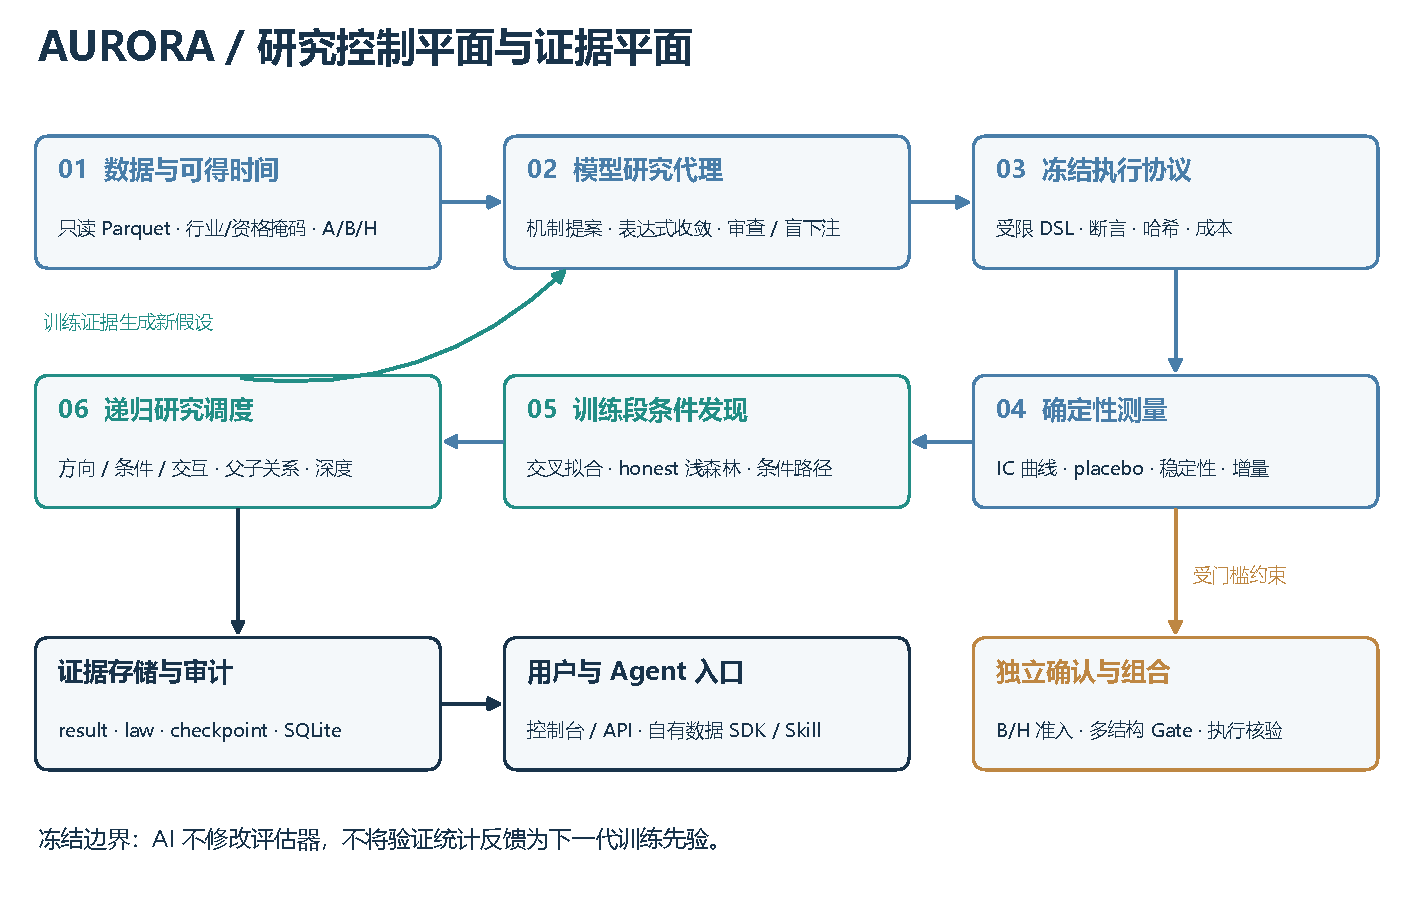
\includegraphics[width=\textwidth]{figures/architecture.pdf}
\caption{AURORA 的研究与产品分层。演化层只能生成新任务，不能改写冻结评估层。}
\label{fig:architecture}
\end{figure}

\subsection{代码模块映射}
\begin{longtable}{p{0.36\textwidth}p{0.56\textwidth}}
\toprule
模块 & 当前职责 \\
\midrule
\code{engine/data.py}, \code{research\_fields.py} & 数据扫描、字段派生、标签构造、行业和竞价质量边界。 \\
\code{engine/config.py} & 日期边界、成本、随机种子、检验规模、模式和 worker 数的冻结配置。 \\
\code{engine/dsl.py}, \code{forms.py}, \code{catalog.py} & 受限表达式编译、结构形式契约、机制家族和可搜索网格。 \\
\code{engine/pipeline.py} & 单结构生命周期、检查点、测量提交、后处理和批次完成。 \\
\code{engine/placebo.py}, \code{blades.py}, \code{metrics.py} & 安慰剂、断言检验、HAC/块 bootstrap、稳定性和成本分析。 \\
\code{engine/discovery.py} & A 段候选筛查、交叉拟合正交化、honest R-learning 浅森林、ICM 交互矩。 \\
\code{engine/discovery\_parallel.py} & fast 模式按时间切分的 Windows spawn 多进程发现。 \\
\code{engine/cycle.py}, \code{continuation.py} & 任务队列、自动演化、父结构继承和续接批次。 \\
\code{engine/llm.py} & DeepSeek proposer、operationalizer、reviewer、bettor、reconciler、inducer 的角色隔离与缓存。 \\
\code{engine/audit.py} & SQLite 事件链、结构冻结、文件哈希和访问凭证。 \\
\code{composition/} & 多结构组合 gate、成分快照和组合回放。 \\
\code{research\_sdk/}, \code{studio\_api.py} & 企业数据上传、格子定义、独立运行和报告导出。 \\
\code{src/}, \code{dashboard\_server.py} & React/Three.js 控制面板、研究进度和 3D 研究场景。 \\
\bottomrule
\end{longtable}

\section{数据平面与时间边界}
\subsection{只读面板}
原始 Parquet 永不被研究过程修改。数据层首先依据日期和证券谓词扫描输入，再构造长表和矩阵双视图：矩阵视图适合滚动字段、分组收益和前端图表，长表视图适合 DSL 结果、森林训练和逐观测审计。

MarketPanel 包含两组对象：
\begin{itemize}[leftmargin=2em]
  \item \code{fields}：只依赖当日及历史的价格、成交、规模、行业、指数快照、波动和估值代理；
  \item \code{labels}：从 T+1 开盘到 T+1+h 开盘生成的未来收益和行业残差标签。
\end{itemize}

字段缺失、无效比率、暖启动不足、行业缺失和异常竞价状态保持为 NaN 或隔离状态，不被静默填成“其他”。字段和缓存身份包含实现源码哈希，避免同一文件大小掩盖代码变化。

\subsection{A/B/H 研究分段}
当前探索数据范围为 2016-07-01 至 2022-06-30。系统还预留确认段 B（2022-07-22 至 2025-07-31）和 holdout 段 H（2025-08-01 至 2026-07-29），但 fast 模式不读取 B/H 作为正式确认依据。

结构内部采用时间顺序：A 段先进行测量和条件搜索；所有搜索候选冻结后，才允许相应的验证检验。训练与验证之间使用 purge，避免未来收益窗口和滚动特征跨边界泄漏。

\section{研究结构：从格子到可证伪档案}
\subsection{Structure 是最小研究单位}
一个 Structure 不是一条表达式，而是一份完整档案：
\begin{equation}
\text{Structure} = (\text{coordinate},\ \text{labels},\ \text{assertions},\ \text{operational},\ \text{lineage},\ \text{freeze hash}).
\end{equation}

\begin{description}[leftmargin=2em]
  \item[coordinate] 机制家族 M1--M10 与结构形式 F1--F7 的坐标。
  \item[labels] 从固定词表选择 agent、friction、mispricing、correction、form 五个槽位。
  \item[assertions] 测量前冻结的 P1、P2、P3 及条件断言；例如符号、峰值窗口、剂量形状和 side condition。
  \item[operational] 同一机制的三个可执行表达式，用于检查收敛效度，降低单表达式过拟合。
  \item[lineage] parent、operator、moderator、donor、depth 和来源记录。
\end{description}

断言状态只有三种：\texttt{hold}（支持）、\texttt{violated}（与预测矛盾）、\texttt{untested}（证据不足）。\texttt{untested} 不被当成失败，也不允许 LLM 根据它编造机制规律。

\subsection{受限 DSL}
表达式通过白名单函数、字段注册表、窗口边界和方向检查编译。编译器阻止：未来字段、未知列、非法窗口、错误量纲、没有可观测事件的事件机制以及未登记的 operator。LLM 只能生成候选规格，不能执行任意 Python。

典型表达式例如：
\begin{lstlisting}
neg(ts_z(ret_1d, 20))
xs_rank(ret_20d)
neg(ts_std(ret_1d, 20))
\end{lstlisting}
这些表达式只是研究候选，不代表已经通过正式确认。

\section{单结构运行管线}
一个结构从提案到归档经过以下阶段：
\begin{enumerate}[leftmargin=2em]
  \item 从 seed 或演化队列取得坐标和父结构。
  \item DeepSeek proposer 根据受控词表和 form contract 生成机制、表达式、方向和峰值范围。
  \item reviewer 检查逻辑可行性；它看不到研究结果。
  \item DSL 编译、字段登记和 convergent orientation 检查。
  \item 生成结构 ID，计算表达式、覆盖和配置指纹。
  \item bettor 在测量前对断言盲下注，概率独立落盘。
  \item 测量 IC、分组曲线、月度曲线、贡献分解、HAC、覆盖和成本。
  \item 运行 placebo、assertion、stability、increment 等检验。
  \item 对探索候选运行条件发现和 ICM 交互检验。
  \item 提交 result、research-factor、daily-ic、contribution 和耗时。
  \item reconciler 只负责把确定性断言结果分类为 aligned/divergent/unresolved；无效响应会被拒绝并可审计恢复。
  \item 根据当前证据生成有限 follow-up，进入下一轮队列。
\end{enumerate}

\begin{figure}[ht]
\centering
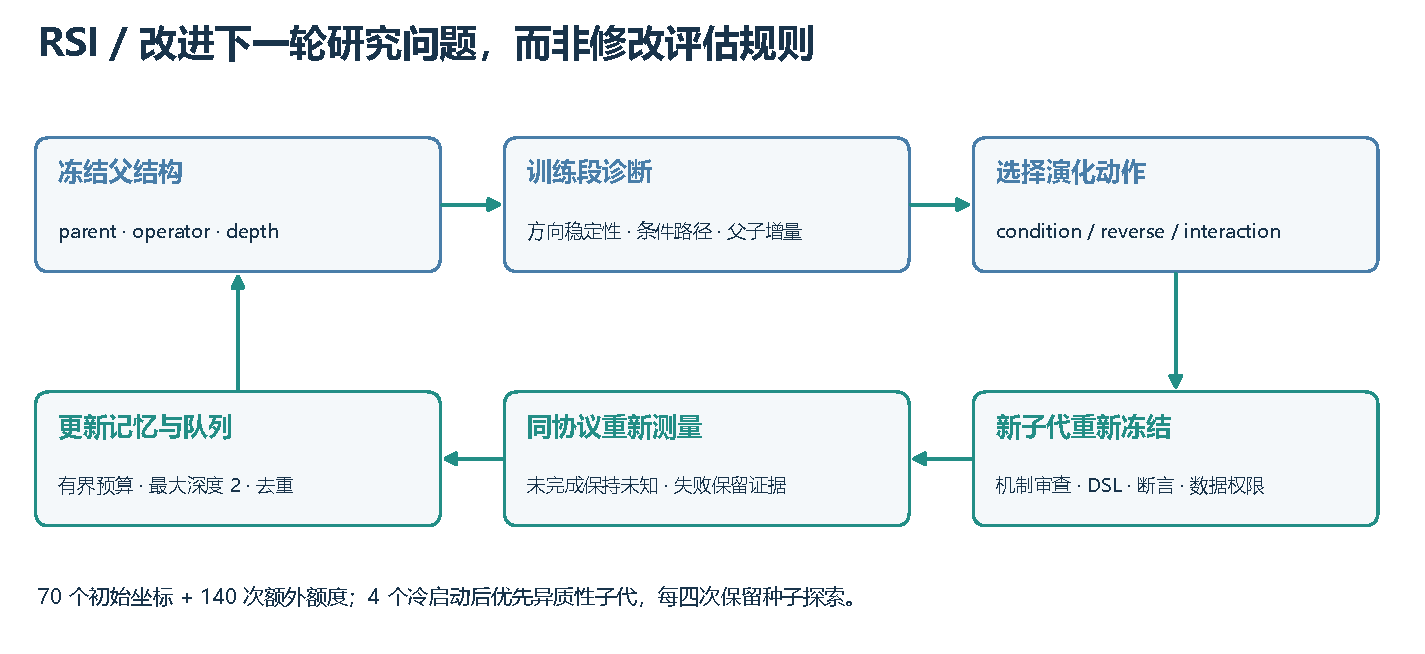
\includegraphics[width=\textwidth]{figures/evolution.pdf}
\caption{AURORA 的 RSI 六步闭环。}
\label{fig:rsi-loop}
\end{figure}

\section{条件发现与多进程森林}
\subsection{为什么需要条件发现}
因子可能只在某个规模、波动、成交或行业状态下成立。AURORA 不允许对全样本任意切分后挑最好的一组，而是先在 A 段进行候选筛查，再使用固定切点、purged split 和独立验证路径检验条件结构。

\subsection{honest R-learning 浅森林}
对每个候选 moderator，系统构造：
\begin{equation}
Y_i = r_i - \widehat{m}(X_i), \qquad D_i = f_i - \widehat{g}(X_i),
\end{equation}
其中 $r_i$ 是未来行业残差收益，$f_i$ 是研究信号，$X_i$ 是规模、波动、成交和行业控制变量。\code{orthogonalize()} 在 purged folds 内拟合稀疏行业指标、三次多项式、样条和 Ridge nuisance model，然后计算残差。

森林只在冻结切点上生成浅树。每棵树使用独立日期块和样本权重，叶子必须满足独立日期和证券覆盖要求。森林输出变量频率、叶子诊断和可审查的条件路径；训练选出的方向与条件进入新假设合同，不被当作独立因果结论或直接反馈验证收益。

\subsection{Windows 多进程实现}
fast 模式的两个时间切分相互独立，因此使用 Windows spawn 子进程并行计算：
\begin{itemize}[leftmargin=2em]
  \item 子进程通过临时 Parquet 读取对应日期范围，不序列化整个 MarketPanel；
  \item 每个进程内的 BLAS、树训练和数值库线程限制为 1，避免嵌套并发；
  \item 按可用内存动态决定实际 worker 数，内存不足时自动退化为串行；
  \item 结果按切分索引合并，保持随机种子、p 值和候选频率与串行结果一致。
\end{itemize}

仓库保留阶段级串行与多进程基准脚本；应以相同冻结结构、数据和线程预算比较耗时，同时检验输出一致性。本次报告没有重新测量全市场耗时，因此不将历史阶段加速比当作当前全流程承诺。

\section{RSI 自动演化闭环}
\subsection{预算与队列}
\code{--full-grid} 当前建立 70 个初始 seed 任务，并预留 140 次自动演化预算，总尝试上限为 210。140 不是预先写死的 140 个表达式，而是后续队列可以消耗的预算；四个冷启动后优先推进异质性子代，每四次保留一次种子探索。实际子代数量取决于训练证据、去重与剩余额度，队列可能提前耗尽。

队列的主要动作及触发来源如下；每次最多提出四个后续假设，实际入队仍受预算、深度与去重限制：
\begin{center}
\begin{tabular}{lll}
\toprule
operator & 含义 & 主要触发条件 \\
\midrule
seed & 网格冷启动 & 尚未研究的机制/形式坐标 \\
condition & 条件区域 & 训练森林的完整条件路径 \\
reverse & 反向假设 & 训练段方向诊断，不直接改变原信号结论 \\
interaction & 跨构件交互 & 冻结父结构与供体的有界交互 \\
horizontal & 同家族换形式 & shape/sign 断言被违反或覆盖不足 \\
cross\_family & 竞争机制 & side 断言被违反 \\
forest & 条件门控 & 森林频率高且探索 p 值满足 fast 阈值 \\
crossover & 条件迁移 & 已有结构支持的 side moderator \\
probe & 记忆引导探针 & inducer 提出有 law 证据的未探索坐标 \\
\bottomrule
\end{tabular}
\end{center}

每个子代继承父任务的问题上下文，而不是父结构的结论。子代必须重新进行表达式编译、断言冻结、盲下注和完整测量，最大 lineage depth 为 2。父结构是失败、未知还是支持，会分别影响可生成的动作；fast 模式允许探索性子代继续验证，但不授予正式 law 或 PASS。

\subsection{训练证据如何转化为下一代合同}
当前 \code{engine/evolution.py} 将方向诊断、条件覆盖和信号组合编码为结构化证据。\code{training\_stop} 使用 $\max(0,\min(800,\lfloor0.55T\rfloor)-\max(15,h+1))$ 作为训练前缀终点；其后保留 purge 间隔再计算后续描述性诊断。选择符号来自训练均值，后续统计不倒灌为该轮方向选择。该拆分仍处于 A 段，不能等同于 B/H 独立确认。

子代动作包括 condition（完整条件路径）、reverse（冻结反向假设）、interaction（跨构件有界交互），以及 horizontal、cross\_family、forest、crossover 与记忆 probe。失败或未知父结构仍可能包含有用的训练异质性线索；这只允许产生新的探索假设，不自动授予有效性。子代记录 parent、donor、operator 与 depth，生成表达式后仍须通过 DSL、机制审查和新冻结。最大深度为 2，队列与模型调用均受预算约束。

\subsection{与无限制自修改的区别}
此处 RSI 的递归对象是\important{研究问题、候选结构、训练条件和搜索分配}。模型不会重写 Python 评估器，也不会自动训练或更新自身权重。执行阶段的数字、断言结果与未完成状态由确定性代码产生；模型负责提出与组织研究解释。这使“下一代研究更具体”成为可审计行为，但是否带来更高质量因子仍需要持续实验验证。

\subsection{组合 Gate 的执行含义}
多结构组合并非将表达式简单相加。系统保留各结构的原覆盖条件，在持仓路径层建立联合规则：等资本并联、冲突区域空仓、至少两个独立构造同向。重复构造需要合并，未知收益不能填零。研究回报代理与 RQAlpha 执行核验分开记录；缺少执行价格或必要确认时，控制台显示失败或等待，不给出虚构净值。

\subsection{性能优化的层次与可测量边界}
\begin{enumerate}[leftmargin=2em]
\item \textbf{共享缓存：} 冻结配置经过规范化后计算缓存身份，父进程和 spawn 子进程使用一致表示，减少重复构建面板。
\item \textbf{切分并行：} 独立进程按日期读取临时 Parquet，内存预算限制 worker 数；原生线程限制为 1，避免 BLAS 与进程池相乘。
\item \textbf{初始网格并行：} Linux 专用 \code{engine.initial\_search} 对不自适应的初始坐标分片，CPU affinity 与共享项目锁约束资源和审计；它不同于递归队列，不能直接等同于完整 RSI 并行运行。
\item \textbf{GPU nuisance 回归：} 可选 CuPy 路径流式累计充分统计量并限制稀疏工作区。它加速回归子步骤，不代表整个森林或全流程均在 GPU 上运行；GPU 依赖与可用显存需要单独配置。
\item \textbf{产品读取：} 前端请求结束后再等待 5 秒轮询，切换批次取消旧请求；默认二维地图，三维按需加载，减少展示对研究资源的占用。
\end{enumerate}
正式、工程和 fast 模式的计算预算不同，不能将 fast 耗时与 formal 精度作无条件等价比较。历史阶段耗时需在同机、同数据、同冻结配置下复核；本次报告更新不额外声称全市场最新加速比。
\subsection{控制指令与研究状态分离}
控制台的 pause/stop 回执表示请求已原子落盘，研究进程在检查点边界生效后才改变实际状态。每批次控制锁串行化操作；重复 resume/restart 不再对存活的已登记 PID 启动第二个恢复进程。已完成批次拒绝继续修改运行状态。

创建恢复进程前，服务先核对代码哈希和 Python/依赖环境，完整数据、模型和产物身份由引擎继续核验。缺少 PID 的外部 CLI 批次不被自动判定为退出。该机制是本机可靠性控制，不是多用户认证或远程运维权限系统；商业部署仍需身份认证、租户隔离、访问策略及受管理的作业服务。

\subsection{RSI 的严格边界}
AURORA 的“自我改进”有四个约束：
\begin{enumerate}[leftmargin=2em]
  \item AI 不能修改 evaluator、时间切分、成本、数据准入和正式确认门槛；
  \item AI 不能读取尚未冻结的验证或 holdout 结果来修改当前结构；
  \item AI 只能提交结构化 JSON，并由 schema、DSL 和审计层拒绝非法结果；
  \item 演化是有限预算的研究搜索，不是无限自我复制或无边界模型升级。
\end{enumerate}

\section{DeepSeek 角色与信息防火墙}
DeepSeek 不是一个拥有完整数据库权限的“自动交易员”，而是五个受限角色：
\begin{description}[leftmargin=2em]
  \item[proposer] 根据坐标、词表、form contract 和父结构先验提出机制规格。
  \item[reviewer] 只审核先验逻辑、字段可用性和形式一致性，不读取结果。
  \item[bettor] 在测量前对断言给出盲先验概率。
  \item[reconciler] 将已经计算好的断言状态分组，不能改变状态。
  \item[inducer] 根据已经落盘的 law 提出 probe 和连接假设，不能宣布确认。
\end{description}

每次请求以 role、context、instruction、model、nonce 和版本形成缓存身份。缓存既提高恢复速度，也让同一请求可复核。2026 年 9 月 8 日第二结构曾收到三个空数组的 reconciler 响应，系统拒绝该响应；恢复脚本保留原响应、使用唯一 nonce 重试，并在确认完整覆盖后恢复运行。这体现了“模型输出可失败，但研究证据不能被默默篡改”的原则。

\section{审计、检查点与可复现性}
\subsection{冻结身份}
每个批次的 identity 包含：
\begin{itemize}[leftmargin=2em]
  \item 配置、日期、成本、随机种子、模式和 worker 上限；
  \item Python 与关键依赖版本；
  \item 输入 Parquet 的文件哈希；
  \item engine 源码哈希；
  \item DeepSeek endpoint/model 的公开配置身份；
  \item discovery 与 Bayesian 开关。
\end{itemize}

如果继续运行时 identity 变化，系统拒绝恢复；如果要改变代码、统计规模或数据范围，必须创建新批次。\code{continue-from} 只继承已验证结构和队列，不把继承结果冒充新批次的独立重复。

\subsection{检查点提交顺序}
结构的测量和结果先写入结构目录，再把 \code{pending\_postprocess} 写入 checkpoint。若 LLM 后处理、记忆刷新或 inducer 失败，恢复时只重做后处理，不重复昂贵的测量和森林。每个恢复事件也进入 SQLite 事件链。

\section{正式、工程与 fast 模式}
\begin{longtable}{p{0.22\textwidth}p{0.22\textwidth}p{0.47\textwidth}}
\toprule
模式 & 主要用途 & 当前协议 \\
\midrule
formal & 正式确认 & bootstrap 1000、placebo 500、森林 500 棵树、20 次切分；需要 B/H 独立确认。 \\
engineering & 工程验收 & 缩小重复次数，验证端到端流程和数据边界。 \\
fast & RSI 闭环与演示 & 全量 A 段、19 次诊断 placebo、30 棵树、2 次切分、多进程；允许探索性子代，但禁止正式 PASS。 \\
\bottomrule
\end{longtable}

fast 的目标是尽快回答“提案、编译、测量、批评、演化、组合和恢复能否闭环”，而不是用缩小的重复次数取得正式统计结论。fast 报告中的 p 值只作为资源分配和研究诊断，不能写成最终因子显著性。

\section{组合 Gate 与多结构研究}
单结构完成后，\code{composition/} 可以按固定完成顺序冻结前 4、8、16 个结构，生成组合 gate 和回放。组合过程不按收益临时挑成分，不把组合结果回写成单结构的验证证据。组合输出包括成分快照、暴露、冲突持仓、成本和执行状态。

这种设计允许研究叙事从“AI 找到一个因子”升级为“AI 形成了可审计的结构组合”：
\begin{enumerate}[leftmargin=2em]
  \item 基础结构提供机制和表达式；
  \item 条件发现提供 gate；
  \item crossover 迁移可复用条件；
  \item composition runner 评估多结构相互作用；
  \item 回放结果仍与正式确认资格分离。
\end{enumerate}

\section{企业 SDK 与控制面板}
\subsection{SDK}
\code{research\_sdk} 面向企业用户提供轻量化入口：
\begin{enumerate}[leftmargin=2em]
  \item 上传 CSV/Parquet 并校验 date、symbol、open、close 和数值字段；
  \item 以 CellSpec 定义机制、表达式和 horizon；
  \item 以 ExperimentSpec 定义 fast/balanced、训练比例、成本、演化开关和预算；
  \item 固定数据哈希、代码哈希和验证边界；
  \item 运行训练段演化、验证 IC、block bootstrap、成本敏感性和相似度检查；
  \item 输出 candidates、factors、daily path、quality status 和 artifact hashes。
\end{enumerate}

轻量 SDK 的 \code{run\_experiment} 使用确定性的训练段变异，记录 \code{llm\_used: false}；不能将其演示为 DeepSeek 完整研究调用。SDK 的输出状态是 \texttt{NEEDS\_REVIEW} 或 \texttt{REPLICATION\_CANDIDATE}，不会把单次用户运行直接包装成正式金融结论。

\subsection{控制面板}
React/Three.js 控制台包含研究队列、运行模式、数据上传、结构卡、进度日志、3D 研究场景、父子血缘、候选表和组合视图。3D 场景的作用是把机制家族、结构形式、代际关系和运行状态可视化，而不是把统计结果装饰成确定结论。前端通过 FastAPI 读取结构化产物，不绕过后端检查直接修改研究状态。

\FloatBarrier
\section{阶段性成果与证据分级}
\subsection{两组来源，各自保留验证口径}
本报告纳入两组已提供证据。第一组为仓库归档的 2026-09-09 A 段 fast 研究快照，来源是 \code{docs/research/2026-09-09-results.json}；第二组为用户提供的 Core Lab 截图，位于 \code{report/}。两者的候选命名、样本长度与统计口径不同，\important{不合并候选总数、不拼接收益、不声称同一次运行}。截图体现研究方法的阶段性应用，其原始数据与可执行日志尚未随图提供。

\begin{table}[ht]
\centering\small
\begin{tabularx}{\textwidth}{lXX}
\toprule
证据层级 & 已观察到什么 & 可以支持什么 \\
\midrule
可读取的归档 JSON & 11 个候选、表达式、IC 区间、父子关系、探索判定 & 对固定快照进行重统计与审查 \\
Core Lab 截图 & 条件因子、父子增量、重复切分、晋级/观察/剔除与规律账本 & 展示研究过程与下一轮候选合同 \\
独立确认与交易验证 & 当前两组材料未提供完成证据 & 不能推断正式 alpha 或实盘收益 \\
\bottomrule
\end{tabularx}
\caption{阶段成果的来源与可支持的结论。}
\end{table}

\subsection{AURORA 归档：研究闭环已有可审查产物}
快照记录 13 次尝试、210 次总额度与 11 个完成候选。其中 6 个为 UNDECIDABLE、5 个为 FAIL，独立确认数为 0。按逐候选 lineage 重计，可见 4 个有父结构的子代，其中 3 个 horizontal、1 个 cross\_family。顶层 evolution 汇总计数与这些逐条记录不一致，因此本报告保留原文件，使用逐候选记录计算子代数，并在制图来源清单中记录差异。

这批产物证明系统可以产出冻结表达式、测量结果、拒绝证据和可追溯的父子结构，而不是已经发现可交易 alpha。C010 的高换手条件是预设条件表达，不能统计为本轮自动森林发现；该归档尚无自动条件规则。C011 的训练反向线索与后续段方向不一致，不能仅凭训练负 IC 宣布稳定反向因子。
\begin{figure}[ht]
\centering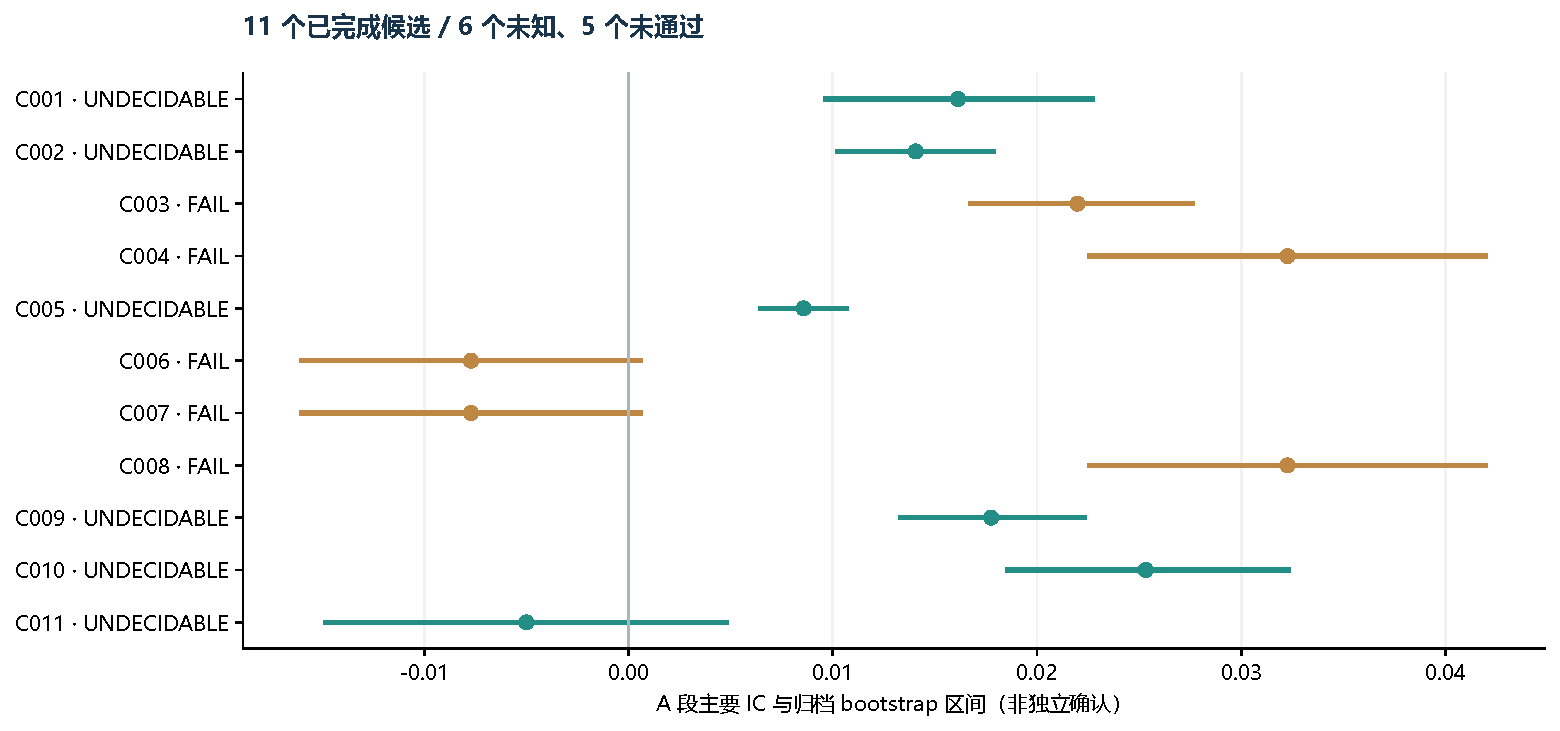
\includegraphics[width=.96\textwidth]{figures/archived_results.pdf}
\caption{归档候选的主要 IC 与原始 bootstrap 区间。绿色为未知，金色为未通过；颜色不代表收益排名。各候选持有期未必相同，图用于证据审查而非严格横向优选。}
\end{figure}

\subsection{Core Lab 案例：条件交互与父子增量}
截图中的候选 \code{CORE170-8EB14F14ED32} 以 \code{pre\_gap\_1d} 为基础，冻结正向、3 日 horizon，并叠加两个区域条件：换手异常相对市场位次不超过 q0.80（图示切点 0.8094），五日收益相对历史位次超过 q0.80（图示切点 0.9）。截图显示第一轮搜索累计两个 gate，说明研究对象从单一信号进入了\important{基础信号与市场状态的交互区域}。

训练区域的父结构 IC 为 0.0210019，条件子结构 IC 为 0.149155，其余区域 IC 为 0.0158302。区域样本数量发生变化，这不是相同样本上净收益提升的证明；其价值在于提出一个明确的下一轮区域假设。训练段仅 25 日、2,201 stock-days，验证段仅 9 日、1,112 stock-days。验证 IC 为 0.0793042、HAC $t$ 为 0.904779，方向虽一致，证据强度仍有限。

\begin{figure}[ht]
\centering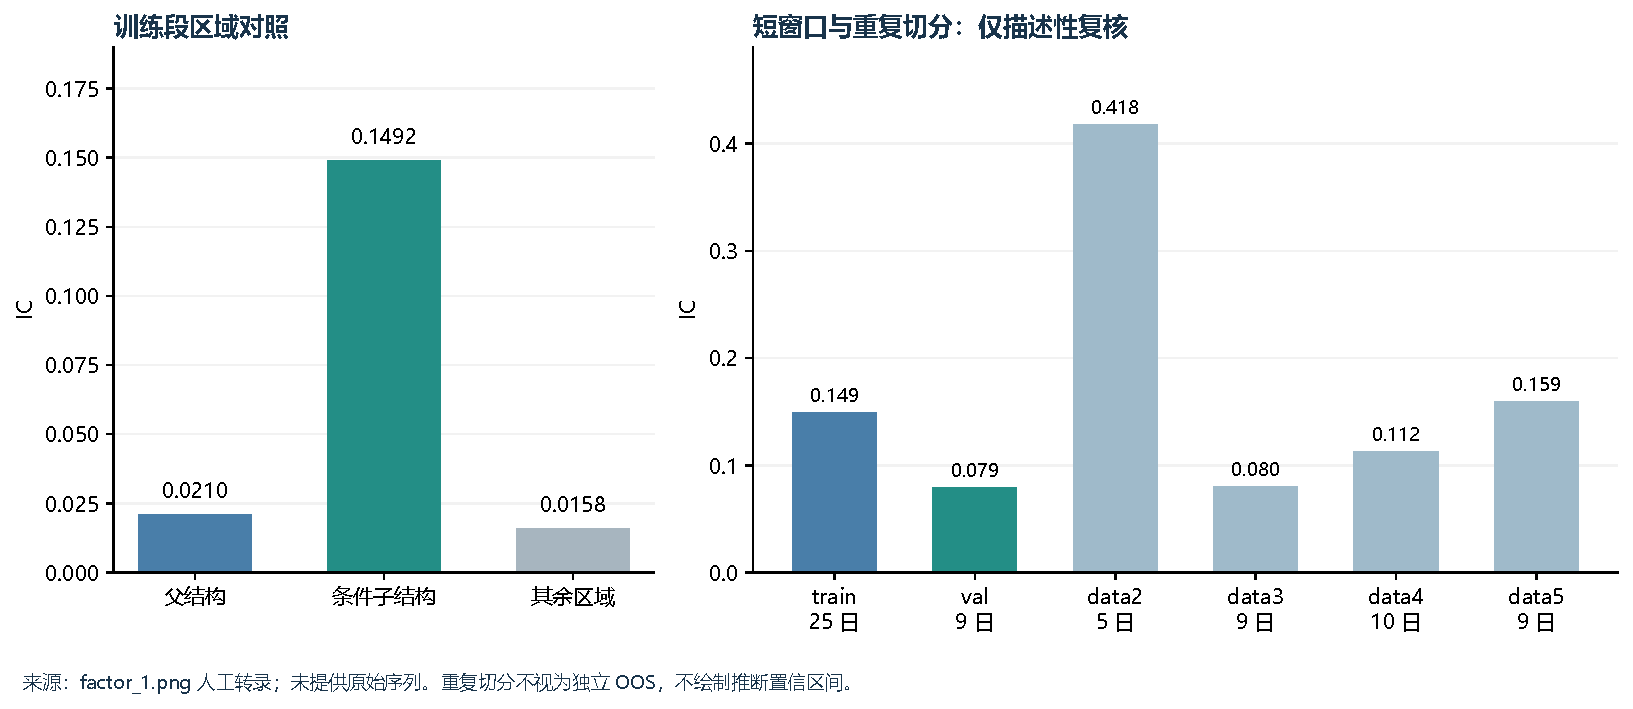
\includegraphics[width=\textwidth]{figures/corelab_case.pdf}
\caption{从用户截图逐值转录的案例。右图 data2--data5 为重复切分标签，不能当作四个独立未见市场。图不补造置信区间，也不把区域 IC 换算为年化收益。}
\end{figure}

\begin{table}[ht]
\centering\small
\begin{tabular}{lrrrr}
\toprule
分段 & IC & HAC $t$ & 交易日 & stock-days \\
\midrule
train & 0.149155 & 2.594850 & 25 & 2201 \\
val & 0.079304 & 0.904779 & 9 & 1112 \\
data2 & 0.417893 & 9.051220 & 5 & 370 \\
data3 & 0.080034 & 0.998685 & 9 & 1341 \\
data4 & 0.112425 & 0.803779 & 10 & 768 \\
data5 & 0.159068 & 1.739080 & 9 & 566 \\
\bottomrule
\end{tabular}
\caption{案例复核值，来源为 factor\_1.png；极短窗口与选择后统计限制其解释范围。}
\end{table}

\subsection{规律账本：把筛选结果反馈为下一轮合同}
\code{factor\_2.png} 的发现后机制解释将该区域描述为消息含义与交易状态/关注结构的交互，并指出它适合作为下一轮 root 合同，而不是事前先验或独立因果结论。\code{law.png} 同时记录 drop 与 observe：例如训练/验证方向翻转、横向强度不足、样本可交易性不足，均有对应理由。

这种记录具有研究价值：失败并非从排行榜消失，而是以边界条件和证据冲突回到下一轮调度。截图里的 promote 表示继续研究的筛选动作，不等于正式 PASS。截图自身也注明 repeated-split 非独立 OOS，以及 CAR、候选内 R-learner 需后续补充；报告沿用这些限制。

\begin{figure}[p]
\centering
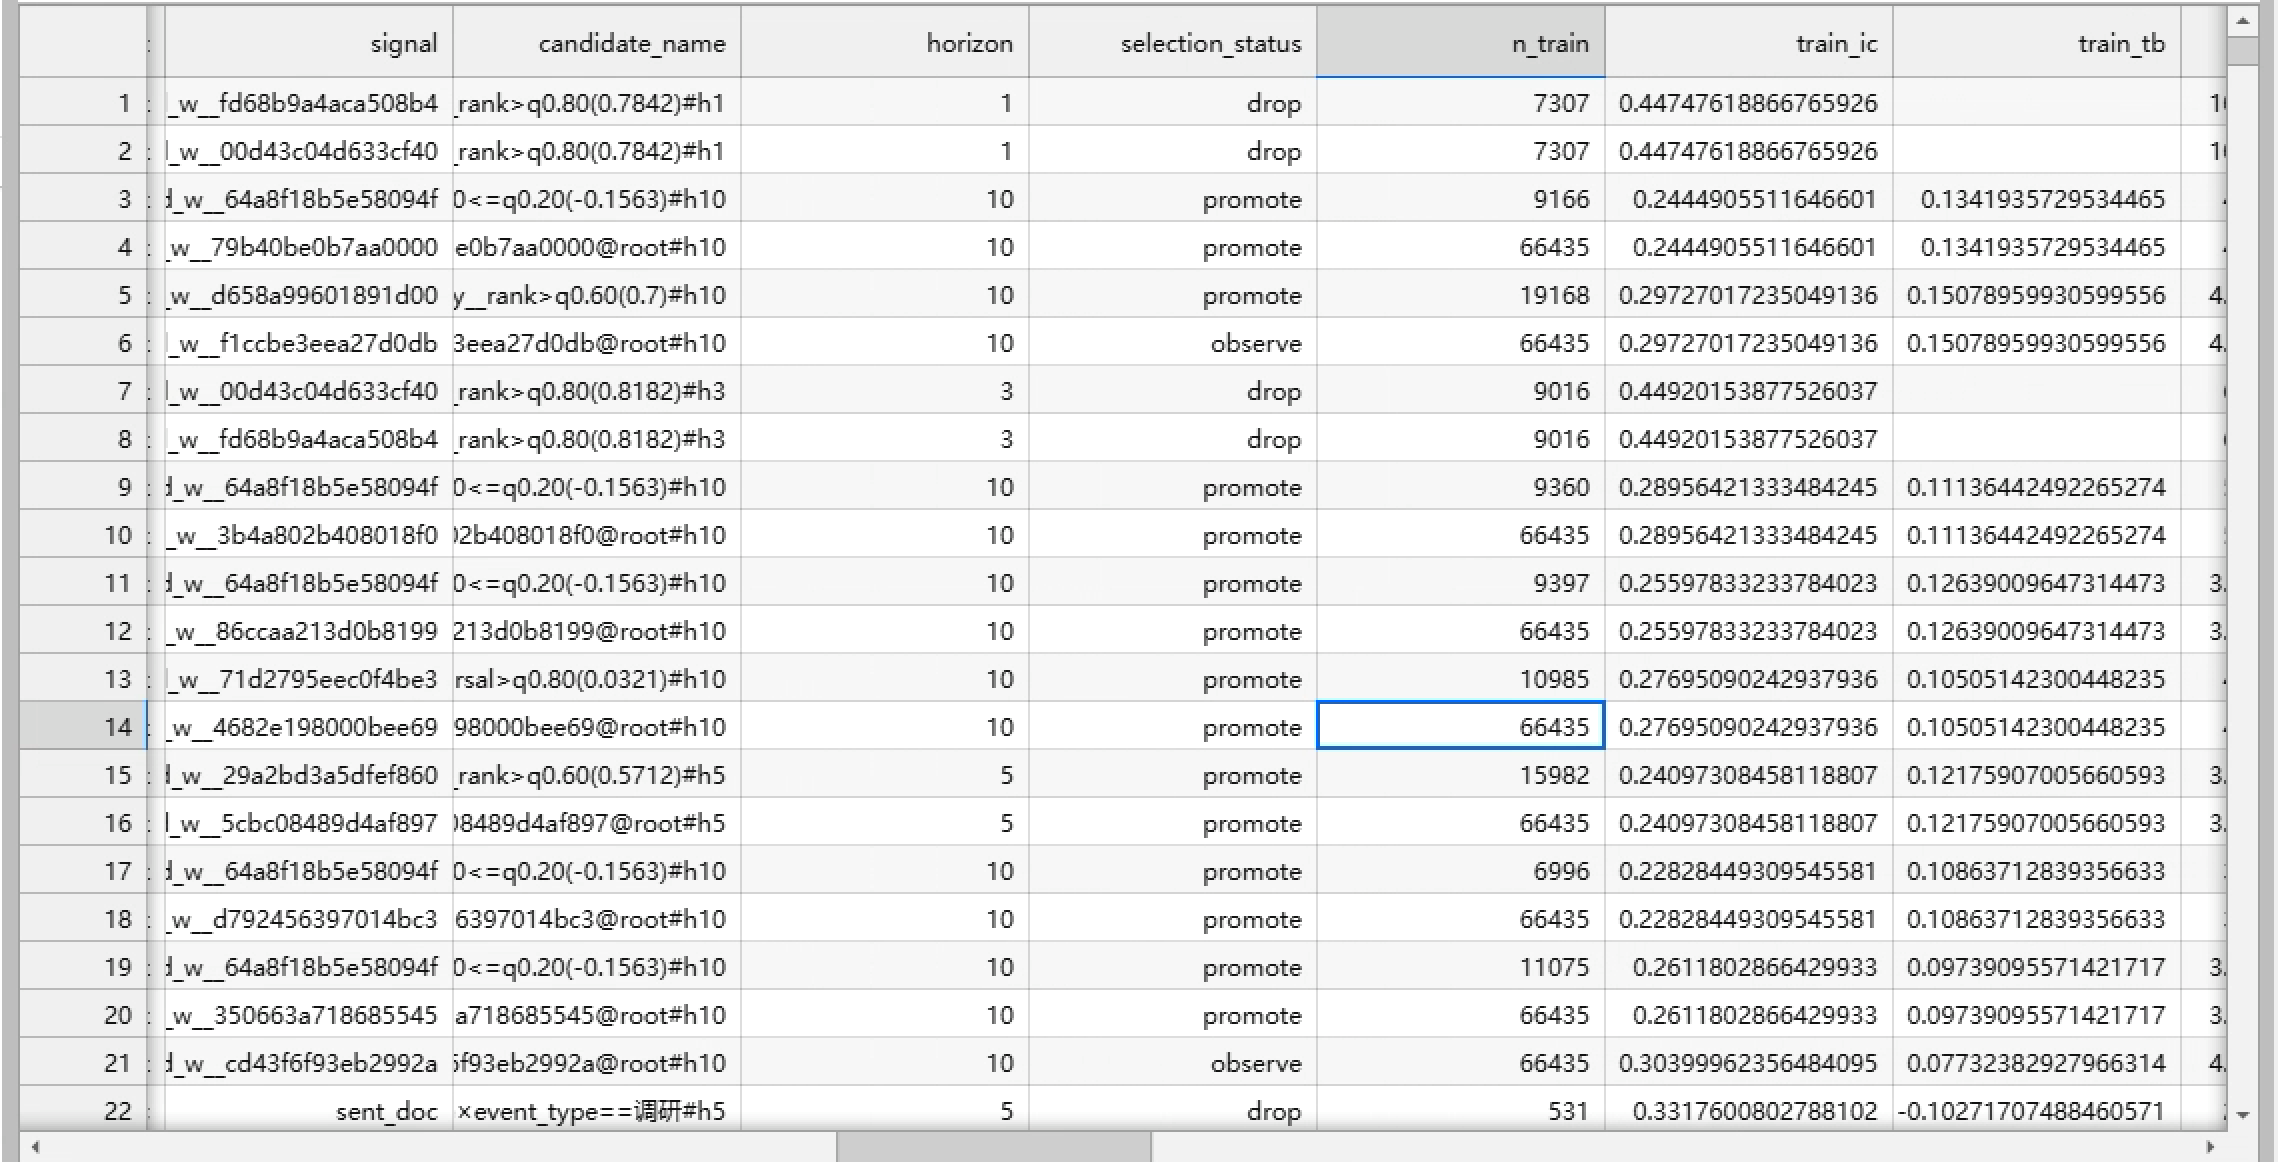
\includegraphics[width=\textwidth,height=.36\textheight,keepaspectratio]{../report/all_factor_show.png}
\caption{原始候选表截屏：同时保留 promote、observe、drop。截图不完整，因此不据此推算候选总量或晋级率。}
\vspace{.8em}
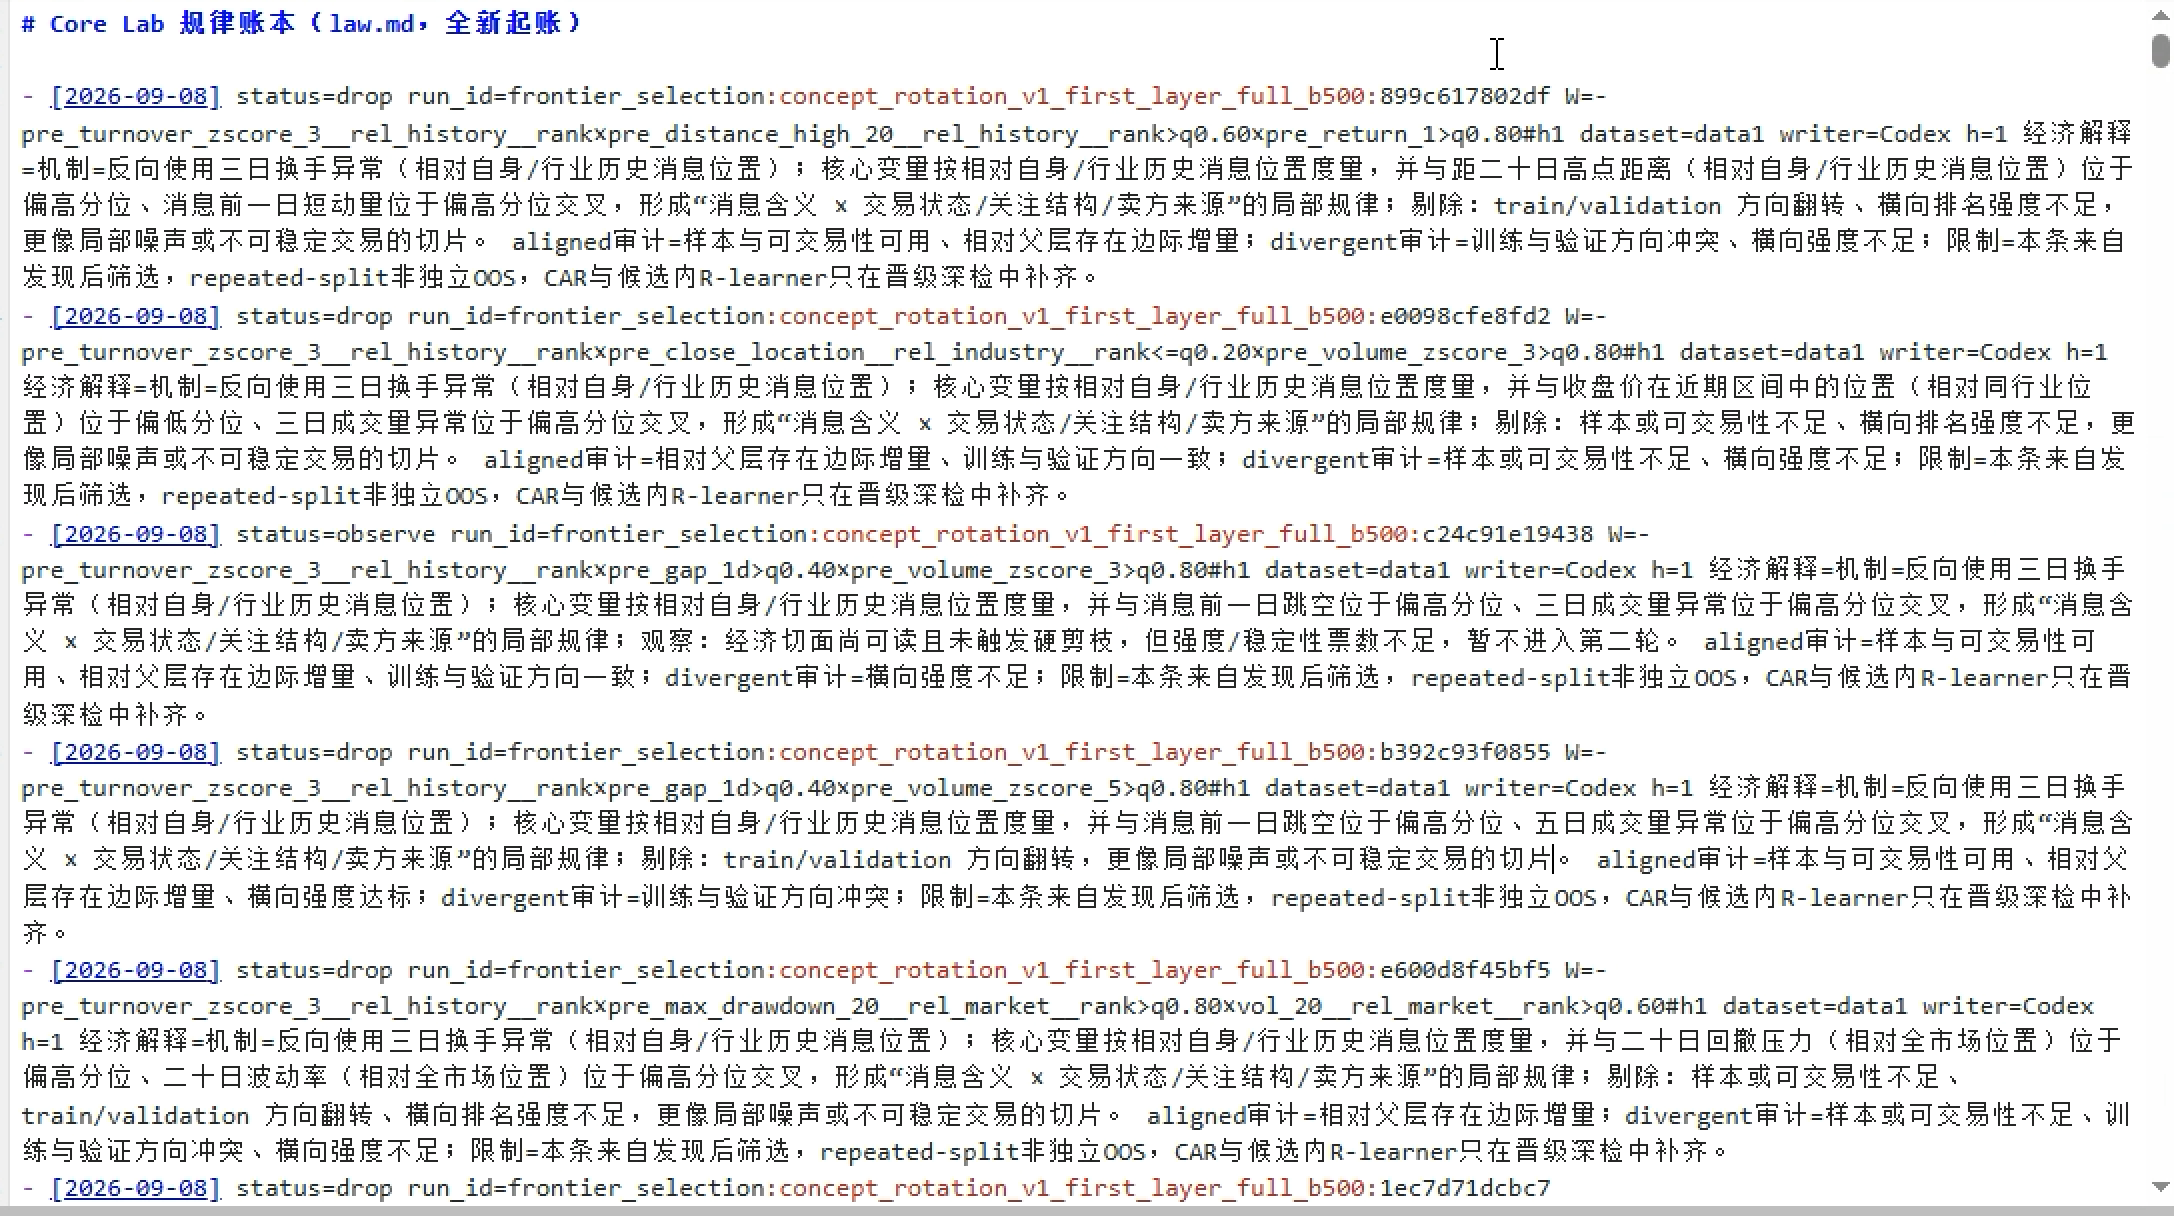
\includegraphics[width=\textwidth,height=.36\textheight,keepaspectratio]{../report/law.png}
\caption{原始规律账本截屏：剔除原因、证据一致与冲突、发现后解释被保留。高清原图随仓库交付。}
\end{figure}
\clearpage
\section{当前实现状态与已知边界}
截至 2026 年 9 月 9 日，仓库已经实现：
\begin{itemize}[leftmargin=2em]
  \item 70 格初始网格、140 次演化预算和最大深度 2 的自动演化队列；
  \item DeepSeek 六角色研究编排与响应缓存；
  \item A 段测量、placebo、断言、稳定性、增量、成本和条件发现；
  \item Windows spawn 多进程发现与串并行一致性测试；
  \item SQLite 审计、哈希冻结、检查点恢复和 reconciler 无效响应恢复；
  \item 组合 gate、回放、企业 SDK、FastAPI 和 3D 控制面板。
\end{itemize}

当前仍需明确的边界包括：
\begin{itemize}[leftmargin=2em]
  \item fast 模式不具备正式确认资格；
  \item 研究区间中的数据隔离、行业来源和竞价数据质量仍会影响正式资格；
  \item 自动演化预算是上限，不保证产生同等数量的有效子代；
  \item LLM 是受限研究代理，不是统计检验器；
  \item 当前组合回放不能替代独立 B/H 确认和真实交易接入。
\end{itemize}

\section{一次完整运行的操作顺序}
\begin{lstlisting}[language=bash]
# 1. fast RSI / autoresearch harness
.venv-research/Scripts/python.exe -u run_engine.py \\
  --fast --full-grid --workers 2 \\
  --industry-policy quarantine \\
  --industry-source exact_intervals \\
  --auction-policy quarantine \\
  --run-id aurora-fast-YYYYMMDD

# 2. 查看批次状态和研究摘要
.venv-research/Scripts/python.exe scripts/summarize_research.py \\
  artifacts/aurora-fast-YYYYMMDD

# 3. 启动控制面板
.venv-research/Scripts/python.exe -m uvicorn dashboard_server:app --host 127.0.0.1 --port 8001
\end{lstlisting}

运行完成后，评审者应首先查看：\code{checkpoint.json}、\code{queue.json}、\code{law.md}、\code{overview.json}、结构目录中的\code{frozen.json/result.json}，以及组合目录中的 gate 和回放报告。这样可以先检查研究过程，再查看候选收益。

\section{结论}
AURORA Alpha Harness 的核心贡献是把“AI 自我改进”从口号变成了受约束的研究协议。AI 可以提出机制、选择下一代任务、组合条件并改进研究路线；评估器、时间切分、成本、数据权限、预算和正式确认门槛仍由 harness 控制。每一次改进都有父结构、操作符、深度、输入哈希、运行状态和失败记录，因此评委可以追问“为什么生成这个结构”“它看到了哪些信息”“哪一步被拒绝”“是否重用了验证结果”，系统能够给出可复核的答案。

这使 AURORA 同时具备三种形态：比赛中的全量 alpha research engine、企业内部的因子研究 SDK，以及面向 AI agent 的 RSI autoresearch harness。它的目标不是让模型无限地产生漂亮表达式，而是让研究方法在有限预算和严格审计下，稳定地产生更清晰、更可证伪、更容易复现的下一轮研究问题。

\appendix
\section{术语表}
\begin{longtable}{p{0.25\textwidth}p{0.65\textwidth}}
\toprule
术语 & 含义 \\
\midrule
RSI & Recursive Self-Improvement，递归自我改进；本项目不是 Relative Strength Index。 \\
Harness & 固定评估协议、权限和审计边界的研究护栏。 \\
Structure & 坐标、标签、断言、表达式、血缘和冻结哈希构成的研究档案。 \\
A/B/H & 探索、确认和 holdout 时间分段。 \\
Placebo & 检查效应是否可能由伪影、前视或巧合造成的诊断。 \\
UNDECIDABLE & 证据不足以判定，不等于 FAIL。 \\
Forest & 在冻结切点和 purged 时间切分上进行条件发现的 honest 浅森林。 \\
Gate & 由 moderator 或条件变量控制结构暴露的门函数。 \\
Lineage depth & 子代距离根结构的演化深度，当前最大为 2。 \\
\bottomrule
\end{longtable}

\clearpage
\section{截图案例原始证据与重建方法}
图中候选编号和数值来自用户提供文件。\par
转录文件：\code{report/evidence-transcription.json}。\par
来源哈希：\code{docs/figures/sources.json}。\par{}原图与转录不一致时以原图为准，并重新核对原始日志。制图使用 Matplotlib，输出嵌入字体的矢量 PDF 和 PNG 预览；流程图由显式节点与连线构建，研究曲线直接读取 JSON，未使用生成式图片替代统计证据。

\begin{figure}[ht]
\centering
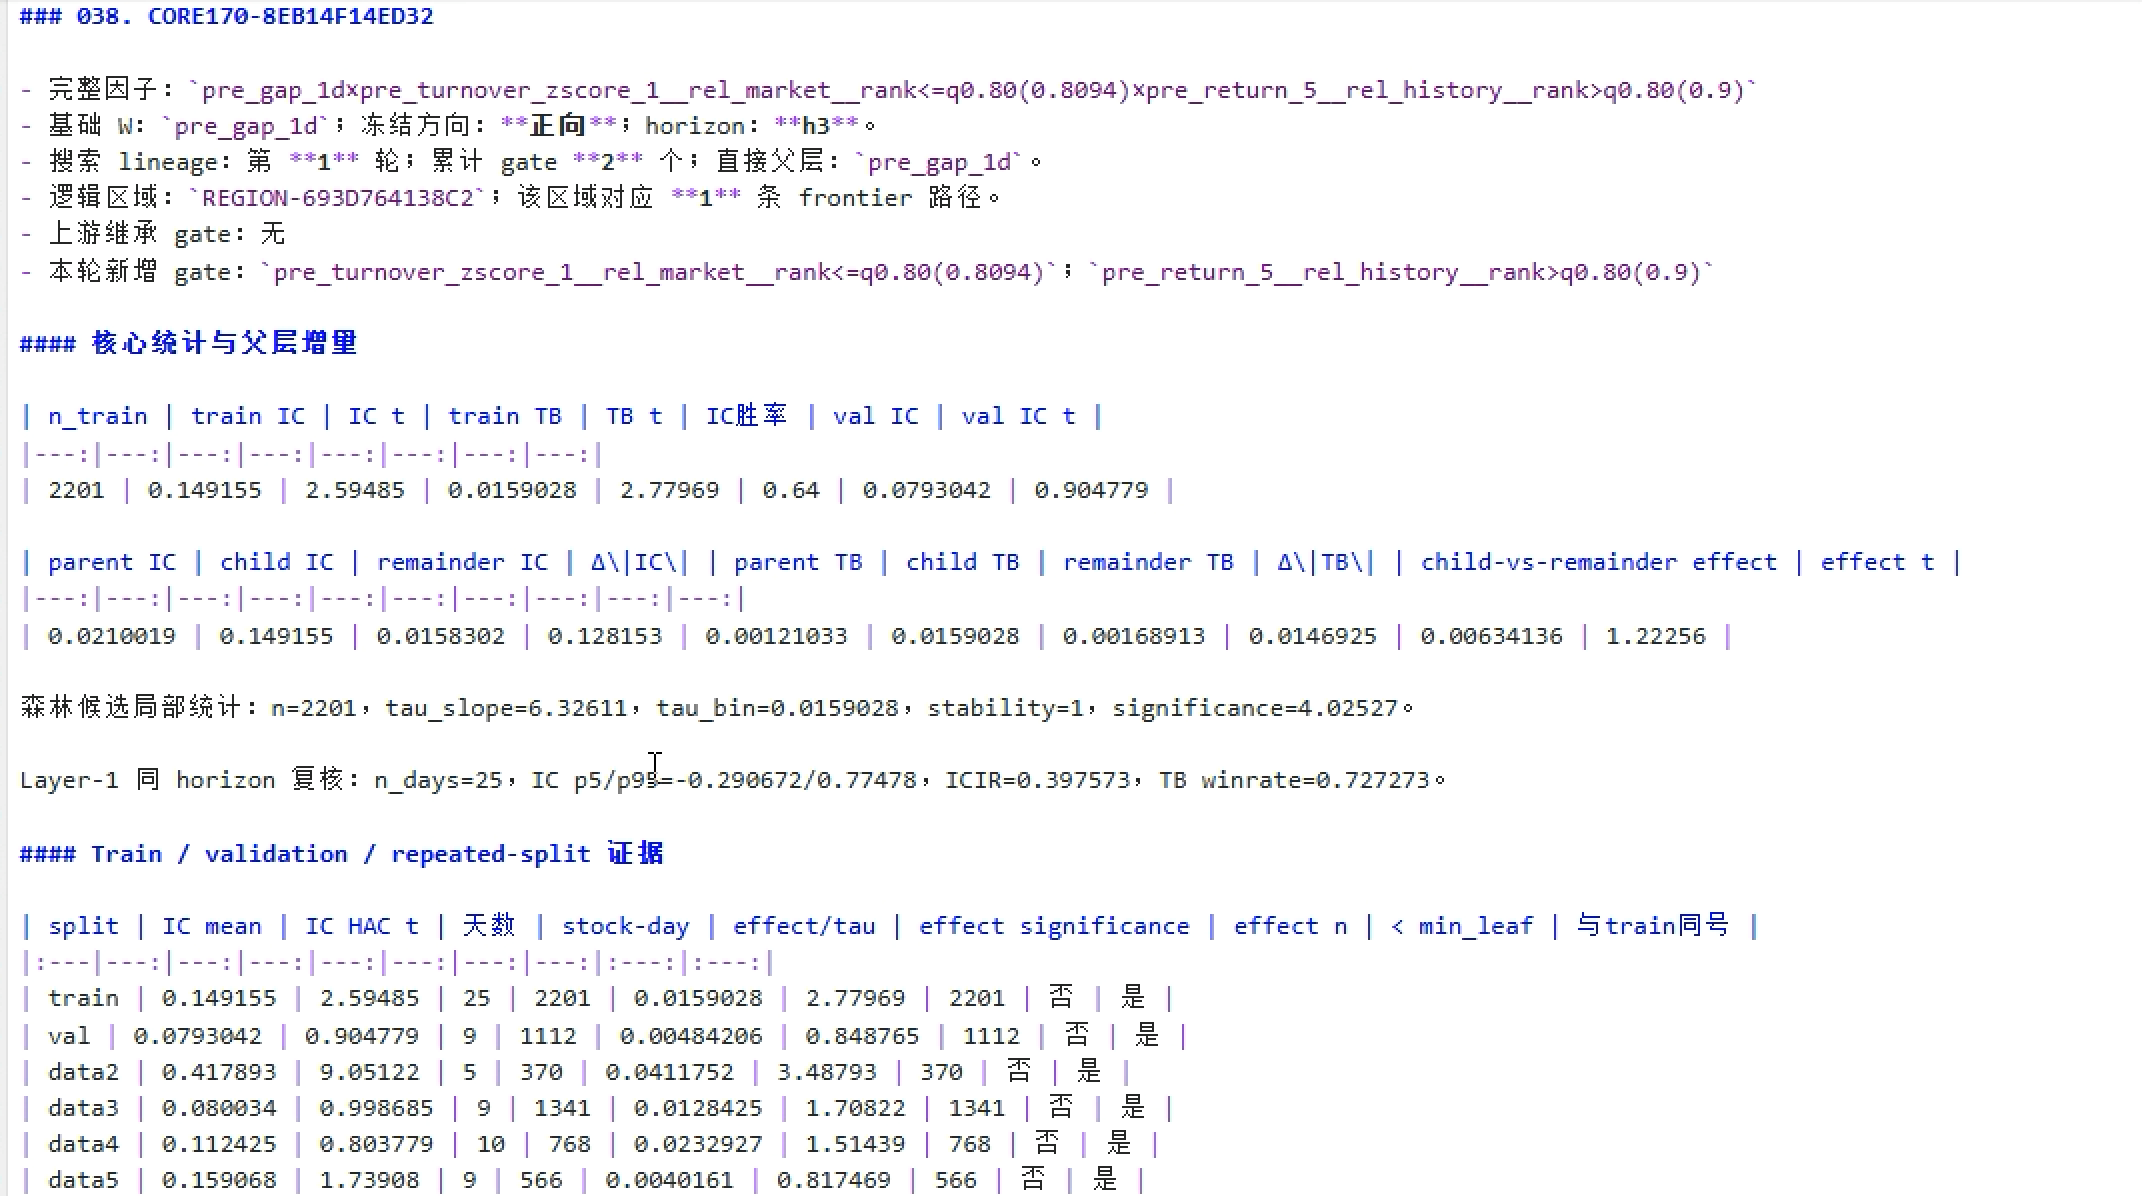
\includegraphics[width=\textwidth,height=.47\textheight,keepaspectratio]{../report/factor_1.png}
\caption{Core Lab 条件候选原始记录。表中的父子增量与多段复核值用于本报告案例重绘。}
\vspace{.7em}
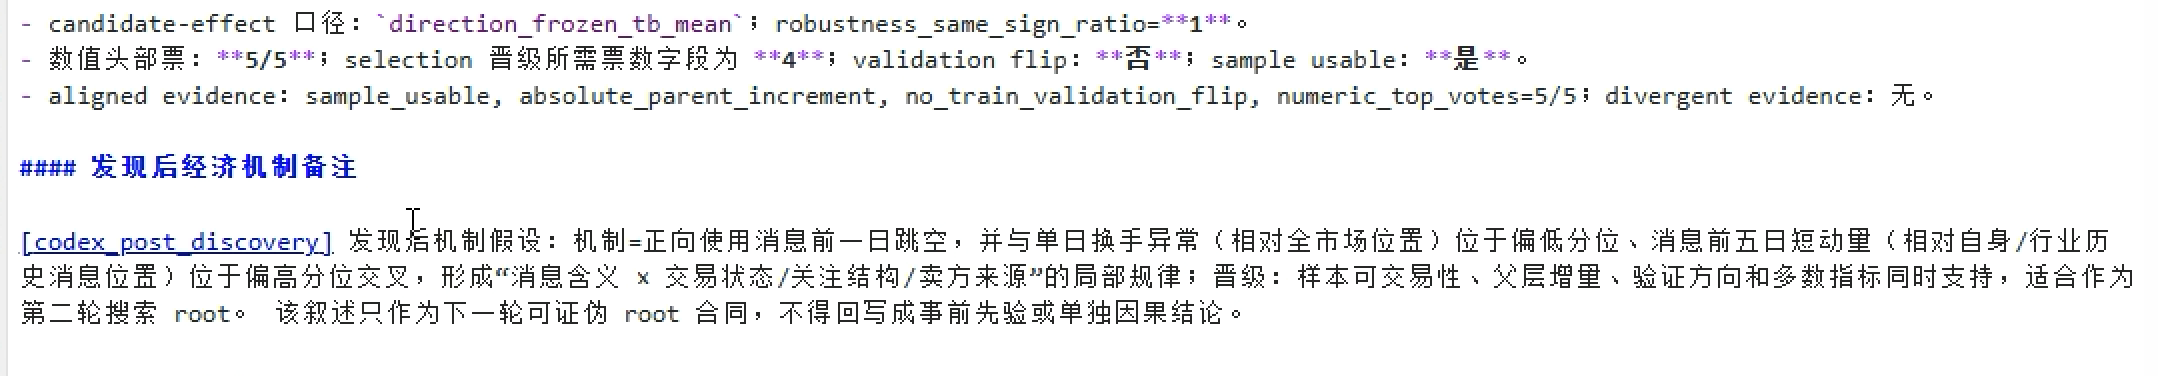
\includegraphics[width=\textwidth]{../report/factor_2.png}
\caption{发现后机制解释的原始记录。其定位是下一轮研究合同，不能回写成事前先验。}
\end{figure}

在仓库根目录运行 \code{scripts/build-report.ps1} 可重新生成四张报告图与 PDF。脚本要求项目 Python、Matplotlib、XeLaTeX 和所用中文字体；遇到制图或编译错误立即退出。Python 测试、浏览器验收与 PDF 构建分别提供工程证据，不代替数据准入、统计校准或市场验证。
\end{document}